\Askhsh{22068}{4}
\begin{ylh}{1}
    \item 1.2. Πρόσθεση και Αφαίρεση Διανυσμάτων.
\end{ylh}
\begin{wrapfigure}[8]{r}{5.5cm}
\centering
\begin{tikzpicture}
    % Ορισμός της αρχής O
    \tkzDefPoint(0,0){O}
    % Ορισμός του σημείου B για το διάνυσμα F2 (στον άξονα x)
    \tkzDefPoint(2.5,0){B} % Επιλέγουμε μήκος 2.5 για καλύτερη οπτική αναπαράσταση
    % Ορισμός του σημείου A για το διάνυσμα F1 (120 μοίρες από το F2)
    \tkzDefPoint(2.5*cos(120), 2.5*sin(120)){A}
    % Ορισμός του σημείου Γ για το διάνυσμα F3 (-120 ή 240 μοίρες από το F2)
    \tkzDefPoint(2.5*cos(-120), 2.5*sin(-120)){C} % Το C αναπαριστά το Γ

    % Σχεδίαση των διανυσμάτων ως παχιά βέλη από το O προς τα A, B, Γ
    \tkzDrawSegments[thick,->](O,A O,B O,C)
    
    % Ετικέτες των σημείων O, A, B, Γ
    \tkzLabelPoint[below left](O){O}
    \tkzLabelPoint[above left](A){A}
    \tkzLabelPoint[right](B){B}
    \tkzLabelPoint[below left](C){$\Gamma$} % Χρήση \Gamma για το ελληνικό γράμμα

    % Ετικέτες των διανυσμάτων F1, F2, F3
    % Η τοποθέτηση επιλέχθηκε ώστε να ταιριάζει όσο το δυνατόν περισσότερο με την αρχική εικόνα
    \tkzLabelLine[pos=0.6,left](O,A){$\vec{F_1}$}
    \tkzLabelLine[pos=0.6,above](O,B){$\vec{F_2}$}
    \tkzLabelLine[pos=0.6,left](O,C){$\vec{F_3}$}
\end{tikzpicture}
\end{wrapfigure}
Σε ένα υλικό σημείο O εφαρμόζονται τρεις δυνάμεις $\vec{F_1}$, $\vec{F_2}$, $\vec{F_3}$ οι οποίες σχηματίζουν ανά δύο γωνία $120^\circ$, έτσι ώστε το υλικό σημείο O να ισορροπεί.
\begin{alist}
\item Ποια σχέση ανάμεσα στα διανύσματα $\vec{F_1}$, $\vec{F_2}$, $\vec{F_3}$ εκφράζει την συνθήκη ισορροπίας; \monades{5}
\item Να αποδείξετε ότι τα διανύσματα $\vec{F_1} + \vec{F_2}$ και $\vec{F_3}$ είναι αντίθετα. \monades{5}
\item Αν A, B, $\Gamma$, $\Delta$ είναι τα πέρατα των διανυσμάτων $\vec{F_1}$, $\vec{F_2}$, $\vec{F_3}$ και $\vec{F_1} + \vec{F_2}$, αντίστοιχα (θεωρούμενων ως διανυσμάτων με αρχή το σημείο O), τότε να αποδείξετε ότι:
    \begin{rlist}
    \item $\wideparen{AO\Delta} = \wideparen{BO\Delta} = 60^\circ$. \monades{5}
    \item $\wideparen{O\Delta B} = 60^\circ$. \monades{5}
    \end{rlist}
\item Να αποδείξετε ότι: $|\vec{F_1}| = |\vec{F_2}| = |\vec{F_3}|$. \monades{5}
\end{alist}